\documentclass[compress,12pt]{beamer}
\usepackage{caption}
\usepackage{subcaption}
\usetheme{Arguelles}
\usepackage{color}
\usepackage{tcolorbox}
\usepackage{xcolor}
\usepackage{booktabs}
\usepackage{algorithm,algpseudocode}
\usepackage{amsfonts, amsmath, amssymb}
\newcommand{\myRed}[1]{\textcolor{red}{#1}}

\title{MATH 512 - Project 3}
\subtitle{}
\event{}
\date{}
\author{Wasif Ahmed, Haoxiang Deng, Jacob Fein-Ashley, Kanav Malhotra, Longzhe Yang}


\begin{document}

\frame[plain]{\titlepage}

\section{Question 1}


% \begin{frame}{Question 1}

%     \begin{itemize}
%         \item We wish to estimate the following expectation $\mathbb{E}[W_3^2 + \sin(W_3) + 2\exp{W_3}]$, where $W_t$ is a standard Wiener process.

%         \item We draw 200,000 pseudo-random samples in the range $[0, \sqrt{3}]$, with each entry as an element $\in W$ ($W$ is a vector).

%         \item Scale $W_3^2 + \sin(W_3) + 2\exp{W_3}$ and we take the sample mean, yielding $\boxed{11.97068421176774}$.

%     \end{itemize}
 
% \end{frame}

% Let 𝑊 𝑡 be a standard Wiener process, that is the drift parameter is zero and the Variance parameter 𝜎2 = 1.
% Suppose that we divide the interval [0,2] 𝑖𝑛𝑡𝑜 𝐿 𝑠𝑢𝑏𝑖𝑛𝑡𝑒𝑟𝑣𝑎𝑙𝑠 [𝑡𝑖, 𝑡𝑖+1], 𝑤𝑖𝑡ℎ 𝑡𝑖 = 𝑖𝛿𝑡 𝑎𝑛𝑑 𝛿𝑡 = 2/𝐿. Let
% 𝑊 𝑖 = 𝑊(𝑡𝑖 ) 𝑎𝑛𝑑 𝛿𝑊 𝑖 = 𝑊 𝑖+1− 𝑊 𝑖. Verify numerically that
% a) ∑ |𝛿𝑊 𝑖|
% 𝐿−1
% 𝑖=0 is unbounded as 𝛿𝑡 goes to zero
% b) ∑ 𝛿𝑊 𝑖
% 2
% 𝐿−1
% 𝑖=0 converges to 2 in probability as 𝛿𝑡 goes to zero

\begin{frame}{Question 1 Overview}
      \begin{itemize}
            \item Let $W_t$ be a standard Wiener process, with drift parameter zero and variance parameter $\sigma^2 = 1$.
            \item We divide the interval $[0,2]$ into $L$ subintervals $[t_i, t_{i+1}]$, where $t_i = i\delta t$ and $\delta t = 2/L$.
            \item Let $W_i = W(t_i)$ and $\delta W_i = W_{i+1} - W_i$.
            \item We verify numerically that:
            \begin{itemize}
                  \item $\sum_{i=0}^{L-1} |\delta W_i|$ is unbounded as $\delta t$ goes to zero.
                  \item $\sum_{i=0}^{L-1} \delta W_i^2$ converges to 2 in probability as $\delta t$ goes to zero.
            \end{itemize}
      \end{itemize}
      
\end{frame}

\begin{frame}{Question 1 Response}
      Refer to Figure~\ref{fig:convergence1}

      \begin{figure}[H]
      \centering
      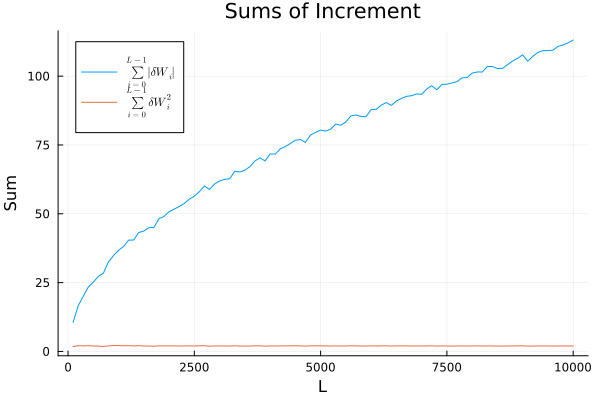
\includegraphics[scale=0.32]{imgs/convergence1.png}
      \caption{Stochastic Plots}
      \label{fig:convergence1}
      \end{figure}

Notice that as the $L$ parameter increases, the $|\delta W_i|$ term is unbounded while $\delta W_i^2$ converges to $2$ in probability.
\end{frame}

% \section*{Question 2}

% \begin{enumerate}
%     \item 
%         \begin{figure}[H]
%             \centering
%             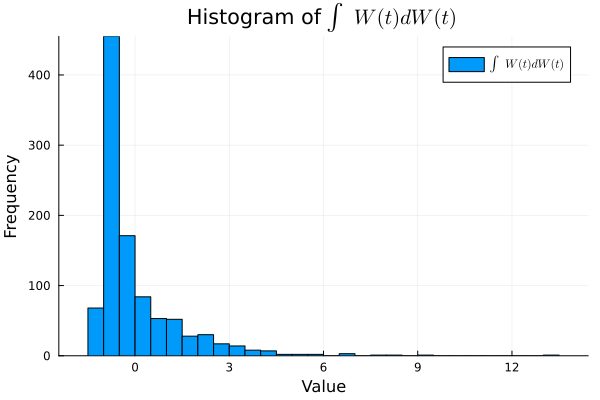
\includegraphics[scale=0.6]{imgs/2a.png}
%             \caption{2a}
%             \label{fig:2a}
%         \end{figure}

%     \item 
%         \begin{figure}[H]
%             \centering
%             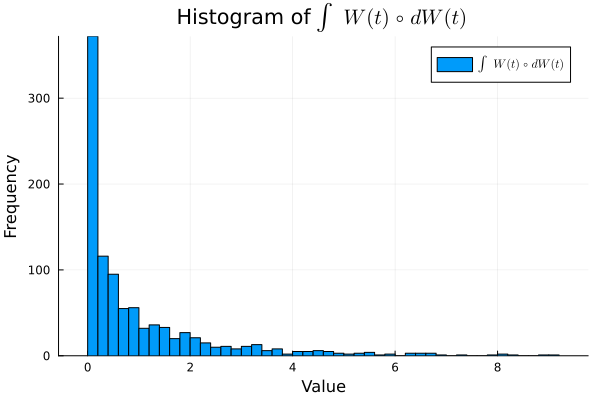
\includegraphics[scale=0.6]{imgs/2b.png}
%             \caption{2b}
%             \label{fig:2b}
%         \end{figure}
%     \item
%         \begin{figure}[H]
%             \centering
%             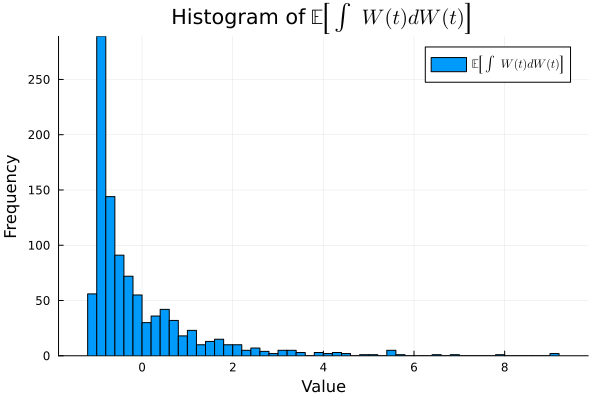
\includegraphics[scale=0.6]{imgs/2c.png}
%             \caption{2c}
%             \label{fig:2c}
%         \end{figure}
%     \item
%         \begin{figure}[H]
%             \centering
%             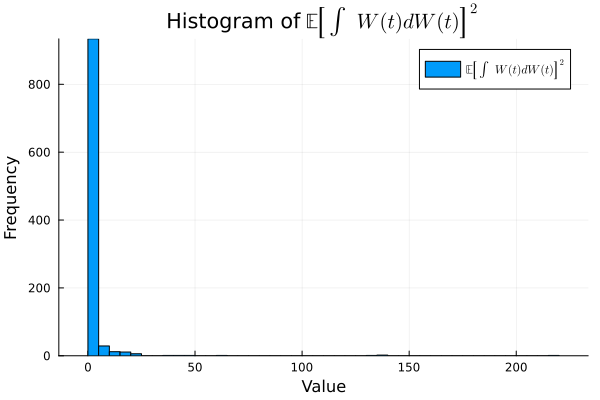
\includegraphics[scale=0.6]{imgs/2d.png}
%             \caption{2d}
%             \label{fig:2d}
%         \end{figure}
%     \item
%         \begin{figure}[H]
%             \centering
%             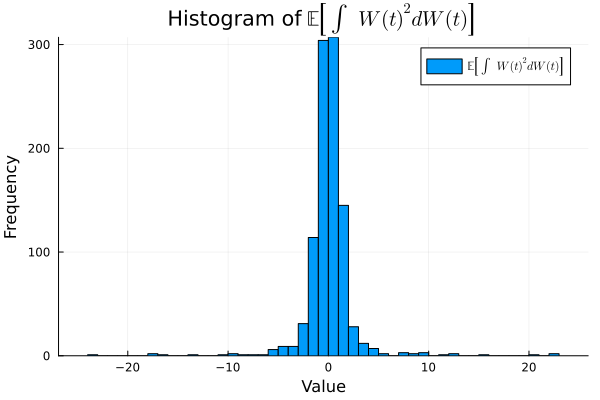
\includegraphics[scale=0.6]{imgs/2e.png}
%             \caption{2e}
%             \label{fig:2e}
%         \end{figure}

%     \item 
%         \begin{figure}[H]
%             \centering
%             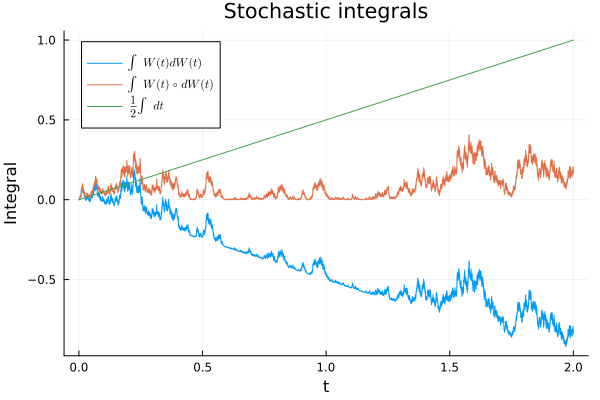
\includegraphics[scale=0.6]{imgs/2f.png}
%             \caption{2f}
%             \label{fig:2f}
%         \end{figure}
% \end{enumerate}

\section{Question 2}
\begin{frame}{Question 2a}
      
% # Evaluate numerically the stochastic integrals
% # a) It𝑜̂ ∫ 𝑊(𝑡)𝑑𝑊(𝑡) on the interval [0,2]

      \begin{figure}[H]
            \centering
            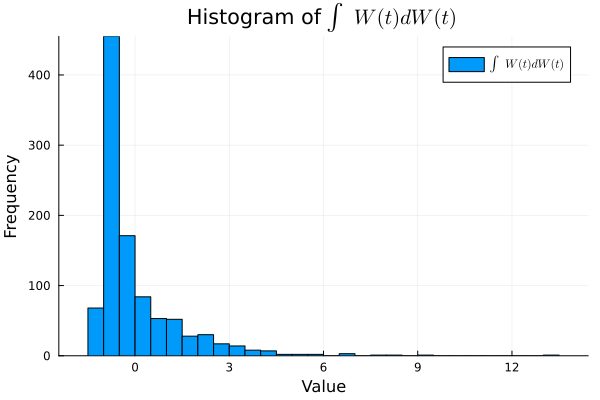
\includegraphics[scale=0.5]{imgs/2a.png}
            \caption{2a}
            \label{fig:2a}
      \end{figure}

\end{frame}

\begin{frame}{Question 2b}
      % # b) Stratonovich ∫ 𝑊(𝑡) ∘ 𝑑𝑊(𝑡) on the interval [0,2]
      \begin{figure}[H]
            \centering
            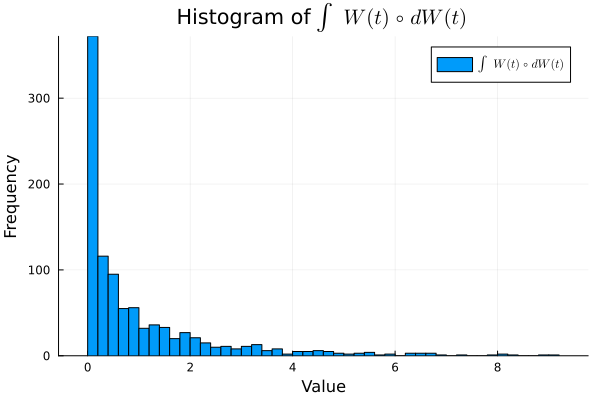
\includegraphics[scale=0.5]{imgs/2b.png}
            \caption{2b}
            \label{fig:2b}
      \end{figure}
\end{frame}

\begin{frame}{Question 2c}
      % # E[∫ 𝑊(𝑡)𝑑𝑊(𝑡)] on the interval [0,2]
      \begin{figure}[H]
            \centering
            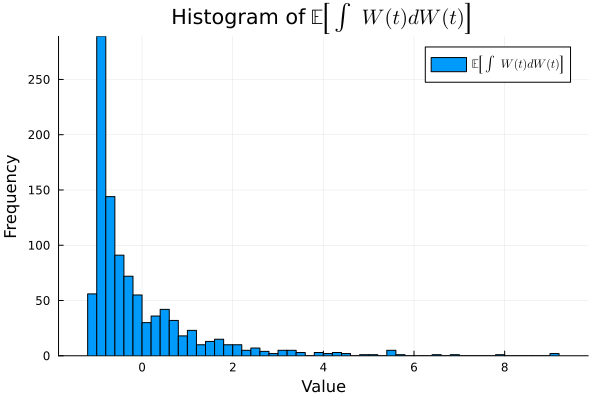
\includegraphics[scale=0.5]{imgs/2c.png}
            \caption{2c}
            \label{fig:2c}
      \end{figure}
\end{frame}

% # E[∫ 𝑊(𝑡)𝑑𝑊(𝑡)]^2 on the interval [0,2]
\begin{frame}{Question 2d}
      \begin{figure}[H]
            \centering
            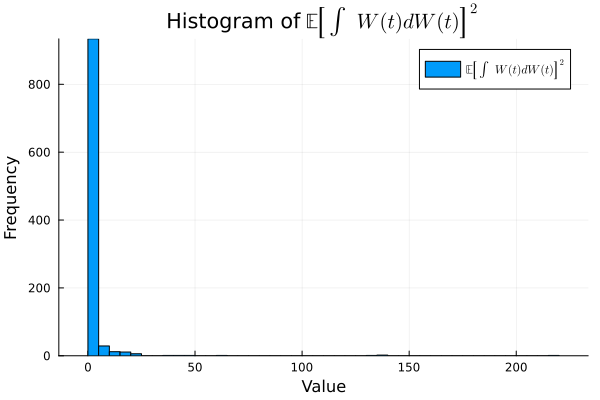
\includegraphics[scale=0.5]{imgs/2d.png}
            \caption{2d}
            \label{fig:2d}
      \end{figure}
\end{frame}

% # E[∫ 𝑊(𝑡)𝑑𝑊(𝑡) ∫ 𝑊(𝑡)𝑑𝑊(𝑡)] on the interval [0,2]
\begin{frame}{Question 2e}
      \begin{figure}[H]
            \centering
            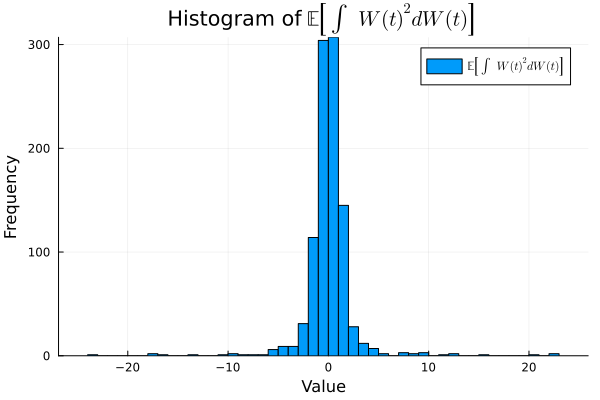
\includegraphics[scale=0.5]{imgs/2e.png}
            \caption{2e}
            \label{fig:2e}
      \end{figure}

\end{frame}

\begin{frame}{Question 2f}
      \begin{figure}[H]
            \centering
            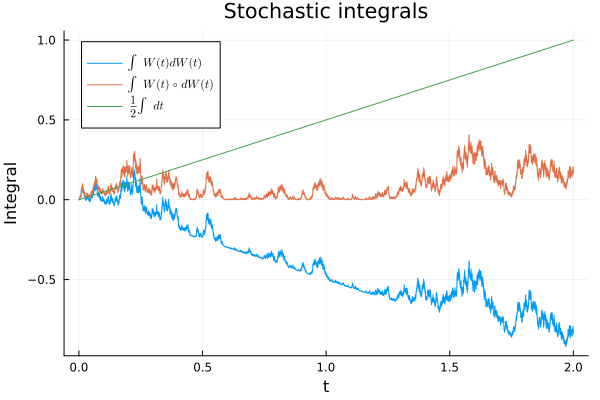
\includegraphics[scale=0.5]{imgs/2f.png}
            \caption{2f}
            \label{fig:2f}
      \end{figure}

\end{frame}

\section{Question 3}




\End
\begin{frame}[plain,standout]
      \centering
      Questions?
\end{frame}

\end{document}
